\documentclass[tikz,border=2pt]{standalone}
\usepackage{amsmath,amssymb}
\usepackage{tikz}
\usepackage{pgfplots}
\pgfplotsset{compat=1.18}

\begin{document}
% Dresses: c = 110, s = 50. The critical ratio beta(p) = (p - c)/(p - s) rises with the price;
% y = 10 stays optimal while F(9) = 0.70 <= beta(p) <= F(10) = 0.85, i.e. 250 <= p <= 450.
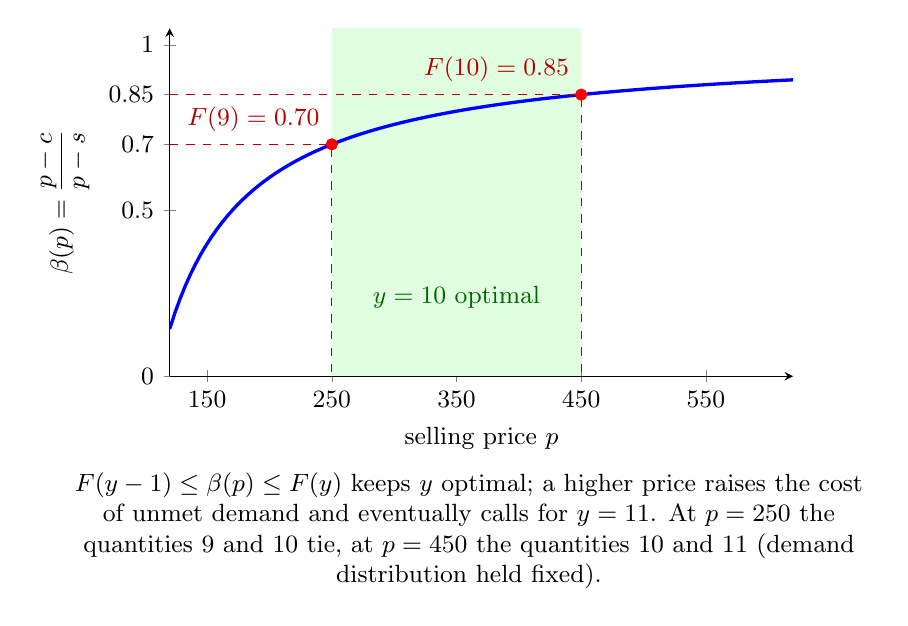
\begin{tikzpicture}
	\begin{axis}[width=9.5cm, height=6cm, xlabel={selling price $p$}, ylabel={$\beta(p)=\dfrac{p-c}{p-s}$}, xmin=120, xmax=620, ymin=0, ymax=1.05, axis lines=left, tick label style={font=\small}, label style={font=\small}, xtick={150,250,350,450,550}, ytick={0,0.5,0.70,0.85,1}, samples=120]
		\fill[green!12] (axis cs:250,0) rectangle (axis cs:450,1.05);
		\addplot[blue, very thick, domain=120:620] {(x-110)/(x-50)};
		\draw[red!70!black, dashed] (axis cs:120,0.70) -- (axis cs:250,0.70) -- (axis cs:250,0);
		\draw[red!70!black, dashed] (axis cs:120,0.85) -- (axis cs:450,0.85) -- (axis cs:450,0);
		\addplot[only marks, mark=*, mark size=2pt, red] coordinates {(250,0.70) (450,0.85)};
		\node[anchor=north, font=\small, green!40!black] at (axis cs:350,0.3) {$y=10$ optimal};
		\node[anchor=south east, font=\small, red!70!black] at (axis cs:248,0.71) {$F(9)=0.70$};
		\node[anchor=south east, font=\small, red!70!black] at (axis cs:448,0.86) {$F(10)=0.85$};
	\end{axis}
	\node[anchor=north, align=flush center, text width=10.2cm, font=\small] at (3.8,-1.1) {$F(y-1)\le\beta(p)\le F(y)$ keeps $y$ optimal; a higher price raises the cost of unmet demand and eventually calls for $y=11$. At $p=250$ the quantities $9$ and $10$ tie, at $p=450$ the quantities $10$ and $11$ (demand distribution held fixed).};
\end{tikzpicture}
\end{document}
